\documentclass[12pt,oneside]{book}
\usepackage[]{biblatex}
\usepackage{xcolor}
\usepackage{graphicx}
\usepackage[]{amsmath,amssymb,amsfonts, amsthm}
\usepackage[]{tcolorbox}
\usepackage[]{thmtools}
\usepackage{geometry}
\usepackage{breqn}
\usepackage{multicol}
\usepackage{varioref}
\usepackage[colorlinks]{hyperref}
\usepackage{cleveref}
\usepackage{physics}
\usepackage{tikz}
\usepackage{mathdots}
\usepackage{yhmath}
\usepackage{cancel}
\usepackage{color}
\usepackage{siunitx}
\usepackage{array}
\usepackage{multirow}
\usepackage{amssymb}
\usepackage{gensymb}
\usepackage{tabularx}
\usepackage{extarrows}
\usepackage{booktabs}
\usetikzlibrary{fadings}
\usetikzlibrary{patterns}
\usetikzlibrary{shadows.blur}
\usetikzlibrary{shapes}

\hypersetup{%
    pdfborder = {1 0 0}
}

\definecolor{titlepagecolor}{cmyk}{1,.60,0,.40}
\definecolor{namecolor}{cmyk}{1,.50,0,.10} 

%-----------------------------------------------------------------
\declaretheorem[name=Lemma,Refname={Lemma,Lemmas}]{lem}
\declaretheorem[name=Example, style=remark,Refname={Example,Examples}]{example}
\declaretheorem[name=Proposition,Refname={Proposition,Proposition}]{prop}
\declaretheorem[name=Theorem,numberwithin=chapter,Refname={Theorem,Theorems}]{thr}\declaretheorem[name=Definition,numberwithin=chapter,Refname={Defintion,Defintions}]{Definition}
\declaretheoremstyle[
    spaceabove=-6pt, 
    spacebelow=6pt, 
    headfont=\normalfont\bfseries, 
    bodyfont = \normalfont,
    postheadspace=1em, 
    qed=$\blacksquare$, 
    headpunct={:}]{myproofstyle} %<---- change this name
\declaretheorem[name=Proof, style=myproofstyle, unnumbered]{Proof}
\declaretheorem[name-Remark, style=remark, numberwithin=chapter]{remark}

%-----------------------------------------------------------------
\newtcolorbox{thmbox}[1][]{colback=white,colframe=red!75!black, arc=0mm}
\newtcolorbox{definitionbox}[1][]{colback=white,colframe=green!75!black, arc=0mm}

%----------------------------------------------------------------
\usepackage{mathtools}

\DeclarePairedDelimiter\abs{\lvert}{\rvert}%
\DeclarePairedDelimiter\norm{\lVert}{\rVert}%

% Swap the definition of \abs* and \norm*, so that \abs
% and \norm resizes the size of the brackets, and the 
% starred version does not.
\makeatletter
\let\oldabs\abs
\def\abs{\@ifstar{\oldabs}{\oldabs*}}
%
\let\oldnorm\norm
\def\norm{\@ifstar{\oldnorm}{\oldnorm*}}
\makeatother
\setlength{\parindent}{0em}

%-----------------------------------------------------------------

\newcommand{\un}[1]{\underline{#1}}
\newcommand{\bwf}[1]{\textbf{#1}}

\newcommand{\S}{\mathbb{S}}
\newcommand{\R}{\mathbb{R}}
\newcommand{\Q}{\mathbb{Q}}
\newcommand{\Z}{\mathbb{Z}}
\newcommand{\C}{\mathbb{C}}

%-----------------------------------------------------------------
\begin{document}
% ----------------------------------------------------------------
\begin{titlepage}
\newgeometry{left=7.5cm} %defines the geometry for the titlepage
\pagecolor{titlepagecolor}
\noindent
\color{white}
\makebox[0pt][l]{\rule{1.3\textwidth}{1pt}}
\par  
\noindent
\textbf{\textsf{Indian Institute of Technology}} \textcolor{namecolor}{\textsf{Bombay}}

\vfill
\noindent
{\huge \textsf{MA 412}}
\vskip\baselineskip\noindent
\textsf{December 2022}
\end{titlepage}
\restoregeometry% restores the geometry
\nopagecolor% Use this to restore the color pages to white
% ----------------------------------------------------------------

\frontmatter
\tableofcontents


\mainmatter
\chapter{Complex Numbers}

\begin{definitionbox}
	\begin{Definition}[Complex Numbers]\label{Complex Numbers}
		We define complex numbers to the ordered pair of real numbers and where addition and multiplication are defined to be as follows:

		\[
			\begin{split}
			\left( a,b \right) + \left( c,d  \right) &= \left( a+c, b+d \right) \\
			\left( a,b \right)  \left( c,d  \right) &= \left( ad-bc, ac+bd \right) 
			\end{split}
		.\]

		It is easily checked that this is in fact a field.
		where the multiplicative identity is $\left( 1,0 \right)$ and the additive identity is $\left( 0, 0 \right) $. 
	\end{Definition}
\end{definitionbox}

If we put $\left( a,b \right) $ as $a+ib$ where $i = (0,1)$ then we can totally abandon the ordered pair notation and perform simple algebra keeping in mind that $i^2 = -1$. \\

Often in copmlex analysis we will be concerned with functions that become $\infty$ when the function approaches a certain given point. To make this notion of distance more formal, we introduce the extended plane  which is the $\C \cup \left\{\infty \right\}  = \C_\infty$

\begin{center}
	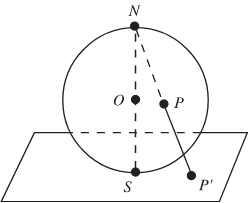
\includegraphics{img/Unknown.png}
\end{center}

Let $N = \left( 0,0,1 \right) $ that is, $N$ is the north pole on $S$. We can identify $\C$ with $\left( x_1, x_2 \right); x_1, x_2 \in  \mathbb{R}$ so that $\C$ cuts $S$ along the equatorial  plane. Now for each point $z \in \C$ consider the straight line in $\mathbb{R}^3$ through $z$ and $N$. This intersects the sphere exactly at one point. $Z \neq N$. If $ \abs{z} > 1$, the point on the sphere must lie in the northern hemisphere and if the point lies in the southern hemisphere, it must lie in the southern hemisphere. It is apparent that as $\abs{z} \to \infty$, $Z$  approaches $N$. Hence, we identify $N$ as the point $\infty$ in $\C_\infty$. \\


Given a point $z$ in $\C$  we can identify the corresponding point $Z$ in $S$ as follows:


\[
	x_1 = \frac{z + \overline{z}}{\abs{z}^2 +1}, x_2= \frac{-i(z - \overline{z})}{\abs{z}^2 +1}, x_3 =  \frac{\abs{z}^2 -1}{\abs{z}^2 +1}
.\] 

Similarly, if we have a point $Z$ in $S / \left\{ \infty \right\} $, the corresponding point in $\C$ as 

\[
z = \frac{x_1 + i x_2}{1-x_3}
.\]
Now we slightly modify the definition of distance in $\C_\infty$ as follows: For $z_1, z_2  \in  \C_\infty$, we have $d(z_1,z_2) = $ the distance between the corresponding points in $\mathbb{R}^3$
Now it is easy to show that distance between two point $z_1, z_2 \in \C$ is equal to the following in $S$:

\[
	\frac{2 \abs{z_1 - z_2}}{\sqrt{1 + z_1^2} \sqrt{1 + z_2^2}} 
.\]

And in a similar way, we get that :

\[
	d\left( z, \infty \right)  =  \frac{2}{\sqrt{1+\abs{z}^2} }
.\]

This correspondence between $S$ and $\C_\infty$ as the stereographic projection.




\chapter{Cauchy-Goursat Theorem}

The Cauchy-Goursat Theorem, which as the name of the chapter suggests, is central to this chapter. So we begin by first stating the theorem itself. 


\begin{definitionbox}
	\begin{Definition}[Cauchy-Goursat Theorem]\label{Cauchy-Goursat Theorem}
		If a function $f$ is analytic at all points interior to and on a simple-closed contour $C$ then
	\[
	\int_{{C}}^{{}} {f\left( z \right) } \: d{z} {} = 0\]

	\end{Definition}
\end{definitionbox}


This theorem is rather hard to prove, so we will be building tools to deal with it for the remainder of the chapter.

Before moving ahead, we would like to define what a \bwf{simply connected} region is.


\begin{definitionbox}
	\begin{Definition}[Simply connected Region]\label{Simply connected Reg}
		A domain $D$ is said to be simply connected if every simple closed contour within it is encloses points of $D$ only. 
	\end{Definition}
\end{definitionbox}

A domain $D$ is said to be \bwf{multiply connected} if it is not simiply connected. 

\begin{example}[Simply Connected Region]
A simple example for simply connected region would be $\C$ itself. Any curve $\left\{\gamma \right \} \in \C$ can only contain points of $\C$ itself. 
\end{example}

\begin{example}[Multiply Connected Region]
	Consider the space $\C^* = \C \setminus \{0\}    $ 


	\begin{center}
		 

\tikzset{every picture/.style={line width=0.75pt}} %set default line width to 0.75pt        

\begin{tikzpicture}[x=0.75pt,y=0.75pt,yscale=-1,xscale=1]
%uncomment if require: \path (0,300); %set diagram left start at 0, and has height of 300

%Shape: Axis 2D [id:dp7089388061410618] 
\draw  (218,223.2) -- (514,223.2)(247.6,27) -- (247.6,245) (507,218.2) -- (514,223.2) -- (507,228.2) (242.6,34) -- (247.6,27) -- (252.6,34)  ;
%Shape: Polygon Curved [id:ds6075001286607652] 
\draw   (204,186) .. controls (224,176) and (314,166) .. (294,186) .. controls (274,206) and (274,216) .. (294,246) .. controls (314,276) and (224,276) .. (204,246) .. controls (184,216) and (184,196) .. (204,186) -- cycle ;
%Shape: Circle [id:dp9295466509908139] 
\draw   (242.49,223.2) .. controls (242.49,220.38) and (244.78,218.09) .. (247.6,218.09) .. controls (250.42,218.09) and (252.71,220.38) .. (252.71,223.2) .. controls (252.71,226.02) and (250.42,228.31) .. (247.6,228.31) .. controls (244.78,228.31) and (242.49,226.02) .. (242.49,223.2) -- cycle ;

% Text Node
\draw (309,158.4) node [anchor=north west][inner sep=0.75pt]    {$\gamma $};
% Text Node
\draw (406,45.4) node [anchor=north west][inner sep=0.75pt]    {$\mathbb{C} \setminus \{0\}$};


\end{tikzpicture}
	\end{center}

	It is apparent that the curve contains 0 $ \not\in \C \setminus \{0\}  $
\end{example}



Let $\gamma_z:= \text{OAB}$. 

Define 
\[
F\left( z \right)  = \int_{{\gamma_z}}^{{}} {f\left(z \right) } \: d{z} {}
.\] 

Then, we have, 



\begin{center}
\tikzset{every picture/.style={line width=0.75pt}} %set default line width to 0.75pt        

\begin{tikzpicture}[x=0.75pt,y=0.75pt,yscale=-1,xscale=1]
%uncomment if require: \path (0,300); %set diagram left start at 0, and has height of 300

%Shape: Circle [id:dp4927592098027098] 
\draw   (205,149) .. controls (205,75.55) and (264.55,16) .. (338,16) .. controls (411.45,16) and (471,75.55) .. (471,149) .. controls (471,222.45) and (411.45,282) .. (338,282) .. controls (264.55,282) and (205,222.45) .. (205,149) -- cycle ;
%Straight Lines [id:da4582551222426777] 
\draw    (338,149) -- (442,149) ;
\draw [shift={(444,149)}, rotate = 180] [color={rgb, 255:red, 0; green, 0; blue, 0 }  ][line width=0.75]    (10.93,-3.29) .. controls (6.95,-1.4) and (3.31,-0.3) .. (0,0) .. controls (3.31,0.3) and (6.95,1.4) .. (10.93,3.29)   ;
%Straight Lines [id:da9233857830894384] 
\draw    (444,149) -- (443.03,81) ;
\draw [shift={(443,79)}, rotate = 89.18] [color={rgb, 255:red, 0; green, 0; blue, 0 }  ][line width=0.75]    (10.93,-3.29) .. controls (6.95,-1.4) and (3.31,-0.3) .. (0,0) .. controls (3.31,0.3) and (6.95,1.4) .. (10.93,3.29)   ;
%Straight Lines [id:da14858467044751889] 
\draw    (391,149) -- (391,112) ;
\draw [shift={(391,110)}, rotate = 90] [color={rgb, 255:red, 0; green, 0; blue, 0 }  ][line width=0.75]    (10.93,-3.29) .. controls (6.95,-1.4) and (3.31,-0.3) .. (0,0) .. controls (3.31,0.3) and (6.95,1.4) .. (10.93,3.29)   ;

% Text Node
\draw (340,152) node [anchor=north west][inner sep=0.75pt]   [align=left] {$\displaystyle 0$};
% Text Node
\draw (446,152) node [anchor=north west][inner sep=0.75pt]   [align=left] {$\displaystyle C$};
% Text Node
\draw (393,152) node [anchor=north west][inner sep=0.75pt]   [align=left] {$\displaystyle A$};
% Text Node
\draw (473,152) node [anchor=north west][inner sep=0.75pt]   [align=left] {$\displaystyle Re\ z$};
% Text Node
\draw (370,93) node [anchor=north west][inner sep=0.75pt]   [align=left] {$\displaystyle B$};
% Text Node
\draw (416,66) node [anchor=north west][inner sep=0.75pt]   [align=left] {$\displaystyle D$};


\end{tikzpicture}
	


\end{center}

Since $f$ is continuous at $z$, 

\[
	f\left( w \right)  = f\left( z \right)  + \phi\left( \omega \right), \omega \in \text{BD}
.\] 

where $\lim_{w \to z} \phi(\omega) = 0$

Therefore, $$\omega \to z, f(\omega) \to  f \left( z \right) $$ \\

Since $g\left( \omega \right) = \omega$ is a primitive for 1,

\[
	\int_{{\text{BD}}}^{{}} {} \: d{\omega} {} = h.
.\] 

Therefore, 


Hell
\end{Proof}\\

\begin{remark}
	The above theorem holds if $f \in  H\left( D \right) $ where $D \subset \C$ is any disk. 
\end{remark}

\begin{remark}
	Let $\Omega \subset \C$ be a disk in $\C$ and if $f \in H\left( \Omega \right) $ then, 

	\[
	\int_{{\gamma}}^{{}} {f\left( z \right) } \: d{z} {} = 0
	.\] 
	for any closed contour $\gamma \subset \Omega$
\end{remark}\\

\begin{remark}
	If $A \subset \C$ and f is holomorphic on $A $ if there is an open set $A \subset U$ such that $f \in  H \left( U \right) $ \\

\end{remark}

\begin{remark}
	If $\gamma$ is an closed contour then $f $ is said to be analytic on and inside $\gamma$ if $f \in H\left( U \right) $

\end{remark}



\begin{definitionbox}
	\begin{Definition}[Domain]\label{Domain}
		A domain $\Omega \subset \C$ is said to be \bwf{simply connected} if for every simple closed curve $\gamma$ lying in $\Omega$, $Int\left( \gamma \right) \subset \Omega$
	\end{Definition}
\end{definitionbox}




\begin{lem}
	Let $f \in H\left( \Omega \right) , \Omega \subset \C$ is simply connected and let $\alpha, \beta \in  \Omega$.

	Then the integral of $f$ along any contour joining $\alpha$	and $\beta$ is same.  
	
\end{lem}

\begin{Proof}
	Let $\gamma_1, \gamma_2$ be two distinct contours joining $\alpha, \beta$. Then, consider the path $\gamma = \gamma_1 + -\left( \gamma_2 \right) $. Then, we have that 
	\[
	\int_{{\gamma}}^{{}} {f\left( z \right) } \: d{z} {} = 0
	.\]
	By Cauchy-Goursat theorem. 
\end{Proof}


\begin{lem}
	Let $\gamma_1$ and $\gamma_2$ be two simple closed contours with same orientations such that $\left\{ \gamma_2 \right\} \subset Int\left( \gamma_1 \right) $. If a function is holomorphic in the closed contour region bounded by $\gamma_1$ and $\gamma_2$, then, 

	\[
	\int_{{\gamma_1}}^{{}} {f\left( z \right) } \: d{z} {} = \int_{{\gamma_2}}^{{}} {f\left( z \right) } \: d{z} {} 
	.\] 
\end{lem}

\begin{center}


\tikzset{every picture/.style={line width=0.75pt}} %set default line width to 0.75pt        

\begin{tikzpicture}[x=0.75pt,y=0.75pt,yscale=-1,xscale=1]
%uncomment if require: \path (0,300); %set diagram left start at 0, and has height of 300

%Shape: Circle [id:dp02448716649342253] 
\draw   (197,145.5) .. controls (197,69.56) and (258.56,8) .. (334.5,8) .. controls (410.44,8) and (472,69.56) .. (472,145.5) .. controls (472,221.44) and (410.44,283) .. (334.5,283) .. controls (258.56,283) and (197,221.44) .. (197,145.5) -- cycle ;
%Shape: Polygon Curved [id:ds8654614936411351] 
\draw   (296,102) .. controls (316,92) and (406,82) .. (386,102) .. controls (366,122) and (366,132) .. (386,162) .. controls (406,192) and (316,192) .. (296,162) .. controls (276,132) and (276,112) .. (296,102) -- cycle ;
%Straight Lines [id:da9010536947679112] 
\draw    (424,42) -- (387.07,100.31) ;
\draw [shift={(386,102)}, rotate = 302.35] [color={rgb, 255:red, 0; green, 0; blue, 0 }  ][line width=0.75]    (10.93,-3.29) .. controls (6.95,-1.4) and (3.31,-0.3) .. (0,0) .. controls (3.31,0.3) and (6.95,1.4) .. (10.93,3.29)   ;
%Shape: Boxed Line [id:dp8382501059640968] 
\draw    (352,185) -- (371.6,282.04) ;
\draw [shift={(372,284)}, rotate = 258.58] [color={rgb, 255:red, 0; green, 0; blue, 0 }  ][line width=0.75]    (10.93,-3.29) .. controls (6.95,-1.4) and (3.31,-0.3) .. (0,0) .. controls (3.31,0.3) and (6.95,1.4) .. (10.93,3.29)   ;
\draw   (355.33,189.67) .. controls (353.5,187.72) and (352.22,185.67) .. (351.48,183.49) .. controls (351.67,185.78) and (351.29,188.17) .. (350.37,190.69) ;
\draw   (422.96,48.08) .. controls (423.32,45.42) and (424.1,43.14) .. (425.33,41.19) .. controls (423.67,42.78) and (421.57,44) .. (419.05,44.87) ;
\draw   (254.25,36.63) .. controls (255.65,34.35) and (257.31,32.58) .. (259.22,31.31) .. controls (257.06,32.08) and (254.65,32.33) .. (251.98,32.1) ;
\draw   (332.82,90.52) .. controls (330.98,92.46) and (329,93.85) .. (326.87,94.7) .. controls (329.14,94.39) and (331.55,94.63) .. (334.11,95.42) ;
\draw   (369.78,136.26) .. controls (371.77,138.06) and (373.21,140) .. (374.12,142.11) .. controls (373.75,139.84) and (373.93,137.43) .. (374.64,134.85) ;

% Text Node
\draw (495,99) node [anchor=north west][inner sep=0.75pt]   [align=left] {$\displaystyle \gamma _{1}$};
% Text Node
\draw (312,188) node [anchor=north west][inner sep=0.75pt]   [align=left] {$\displaystyle \gamma _{2}$};
% Text Node
\draw (352,61) node [anchor=north west][inner sep=0.75pt]   [align=left] {$\displaystyle A$};
% Text Node
\draw (434,22) node [anchor=north west][inner sep=0.75pt]   [align=left] {$\displaystyle B$};
% Text Node
\draw (337.5,159.5) node [anchor=north west][inner sep=0.75pt]   [align=left] {$\displaystyle C$};
% Text Node
\draw (407,271) node [anchor=north west][inner sep=0.75pt]   [align=left] {$\displaystyle D$};
% Text Node
\draw (478,175) node [anchor=north west][inner sep=0.75pt]   [align=left] {$\displaystyle E$};
% Text Node
\draw (176,164) node [anchor=north west][inner sep=0.75pt]   [align=left] {$\displaystyle F$};
% Text Node
\draw (256,113) node [anchor=north west][inner sep=0.75pt]   [align=left] {$\displaystyle G$};
% Text Node
\draw (403,162.4) node [anchor=north west][inner sep=0.75pt]    {$H$};


\end{tikzpicture}	

\end{center}


\begin{thmbox}
	\begin{thr}[Cauchy's Integral Formula]
		Let $\gamma$ be a simple closed contour, and let $z\in  Int\left( \gamma \right) $. If $f$ is analytic on and inside $\gamma$, then, 

		\[
		f\left( z_0 \right)  = \frac{1}{2 \pi i} \int_{{\gamma}}^{{}} {\frac{f\left( z \right)}{z-z_0} } \: d{z} {}
		.\] 
	\end{thr}
\end{thmbox}

\begin{Proof}
	Witout loss of generality, let $\gamma$ be  psotively orineted. Since $f$ is continuous at $z_0$, $\forall \epsilon >0, \exists \delta >0$ such that, 

	\[
		\abs*{z - z_0} < \delta \implies \abs*{f\left( z \right) - f\left( z_0 \right) } < \epsilon 
	.\] 

	Set $\gamma_1:= \abs{z-z_0} = r$, where $0<r<\delta$, Simple Circle positively oriented. 

	The function $\frac{f\left( z \right) }{z-z_0}$ is anlyatic in the closed annular region bounded by $\gamma$ andd $\gamma_1$. Then, by the previous lemma, we have, 

	\[
	\int_{{\gamma}}^{{}} {\frac{f\left( z \right) }{z-z_0}} \: d{z} {} = \[
	\int_{{\gamma_1}}^{{}} {\frac{f\left( z \right) }{z-z_0}} \: d{z} {} 
	.\] 


	Now, we can write the corresponding integral as follows:

	\[
	\int_{{\gamma_1}}^{{}} {\frac{f\left( z \right) }{z-z_0}} \: d{z} {}  = \int_{{\gamma_1}}^{{}} {\frac{f\left( z \right) - f\left( z_0 \right)  }{z-z_0}} \: d{z} {} + \int_{{\gamma_1}}^{{}} {\frac{f\left( z_0 \right) }{z-z_0}} \: d{z} {} 

	Now, 
	\[
		\abs*{ \int_{{\gamma_1}}^{{}} {\frac{f\left( z \right) - f\left( z_0 \right)  }{z-z_0}} \: d{z} {}} \le  \frac{\epsilon}{r}  (2 \pi r)  $
	.\] 

	Hence the first term vanishes as $\epsilon>0$ 

	Now the second term is:

	\[
	\begin{split}
		\int_{{\gamma_1}}^{{}} {\frac{f\left( z_0 \right) }{z-z_0}} \: d{z} {}  &= f\left( z_0 \right) \int_{{\gamma_1}}^{{}} {\frac{1}{z-z_0}} \: d{z} {} \\							&= f\left( z_0 \right) 2 \pi i 
	\end{split}
	.\] 

	Hence, we have that 

	\[
	\[
	\begin{split}
		\frac{1}{2 \pi i}\int_{{\gamma}}^{{}} {f\left( z \right) } \: d{z} {} &= \int_{{\gamma_1}}^{{}} {f\left( z \right) } \: d{z} {} \\ 
										      &=  \frac{f \left( z_0 \right)}{2 \pi i} 2 \pi i = f\left( z_0 \right)  \\
	\end{split}
	.\] 
\end{Proof}


hell








\end{document}
